\documentclass{article}
\usepackage{graphicx}
\usepackage{fullpage}
\usepackage{booktabs}
\usepackage{amsmath}
\usepackage{amsthm}
\usepackage{xspace}
\usepackage{multirow}
\usepackage{algorithm}
\usepackage{algpseudocode}
%
\graphicspath{{figures/}}
%
\theoremstyle{definition}
\newtheorem{definition}{Definition}
%
\newcommand{\model}{\ensuremath{\mathrm{M}}\xspace}
\newcommand{\sd}{\ensuremath{\mathrm{SD}}\xspace}
\newcommand{\comps}{\ensuremath{\mathrm{COMPS}}\xspace}
\newcommand{\pr}[1]{\ensuremath{\mbox{Pr}(#1)}}

%
\title{Stochastic and Quantum Algorithms for Model-Based Diagnosis of Digital Circuits}
%
% Title for submission to Science: Quantum Speedup = Diagnostic Optimality
%
\author{@todo}
%
\begin{document}
\maketitle
\section{Introduction}

\section{Definitions}
%
This section provides the basic framework for the algorithms we design
and analyze.
%
\begin{definition}[Basis]
  %
  A basis $\mathcal{B}$ is a set of single-output Boolean functions
  $\{B_1, B_2, \ldots, B_n\}$.
  %
\end{definition}
%
A basis can be constructed from the common logic-gate types AND, OR,
NAND, NOR, XOR, inverter, and buffer as the $F_1, F_2, \ldots, F_n$
subformulas. The AND, OR, NAND, and NOR gates may have more than two
inputs. Figure~\ref{fig:basis} shows these logic gates
pictographically.
%
\begin{figure}[htb]
\centering \includegraphics{basis.mps}
\caption{Pictographic representation of common logic
  gates\label{fig:basis}}
\end{figure}
\par
%
In this article we use the common propositional logic connectives:
$\wedge$, $\vee$, $\oplus$, $\neg$, $\rightarrow$, and
$\leftrightarrow$. The logical connectives implication ($\rightarrow$)
and equivalence ($\leftrightarrow$) do not appear in the circuits we
are diagnosing and are not part of the basis. The Boolean formula that
is equivalent to an AND gate, for example, is $a \wedge b$. The
semantics of all this is the usual one and is explained in any
introductory logic or VLSI design book.
\par
Logic circuits are designed by drawing gates from the basis and
connecting them with wires. Wires are represented as variables. A
well-formed logic-circuit design is a Direct Acyclic Graph
(DAG). There are no hanging edges in the DAG (that would be a
violation of the common definition for a DAG). We work with connected
DAGs only. If somewhere in our algorithms a DAG gets disconnected, we
remove the orphan or treat the two disconnected DAGs separately.
%
\begin{definition}[Boolean Circuit]
  %
  Given a basis $\mathcal{B}$, a Boolean circuit $\model(\mathcal{B})
  = \langle{V \cup \{I^\star, O^\star\}, E}\rangle$ is a DAG in which
  each edge $e \in E$ is a variable, each node $v \in V$ is a Boolean
  function drawn from $\mathcal{B}$, $I^\star$ is a primary input
  source, and $O^\star$ is a primary output sink.
  %
\end{definition}
%
The special primary input source and primary output sink nodes are not
normally drawn in a circuit diagram. The edges that are adjacent to
$I^\star$ are the primary inputs and the edges that are adjacent to
$O^\star$ are the primary outputs.
\par
Implementation of Boolean functions as electric circuits perform
useful function such as adding or multiplying numbers, detecting or
correcting errors, etc. Combined with memory elements (flip-flops)
they become the foundation of most modern computing (except quantum).
\par
In this article we will use the circuit shown in
figure~\ref{fig:adder} as a running example. Its function is to add-up
two two-bit numbers in binary. The result is a two-bit sum and a carry
bit.
%
\begin{figure}[htb]
\centering
\includegraphics{adder_2.mps}
\caption{$2$-bit adder\label{fig:adder}}
\end{figure}
\par
%
A Boolean circuit, as defined, has no provisions for failure. We can
allow parts of a circuit to fail by introducing extra fault variables
and extra elementary failure functions (constraints).
%
\begin{definition}[Fault-Augmented Model]\label{def:sd}
  %
  Given a basis $\mathcal{B}$, a Boolean circuit $\model(\mathcal{B})$
  and a second fault-augmented basis $\mathcal{B}^\star$, a
  fault-augmented model $\sd(\mathcal{B}, \mathcal{B^\star})$ is
  defined as the ordered triple $\langle{\comps, V, E, F}\rangle$
  where $\comps = \{f_1, f_2, \ldots, f_n\}$, $n = \left|V\right|$,
  and $F$ is a mapping $F: \mathcal{B} \rightarrow \mathcal{B}^\star$.
  %
\end{definition}
%
Definition~\ref{def:sd} allows us to add a fault variable to each
logic gate, and depending on the value of the fault variable to allow
either the original (intended) behavior of the gate or some specified
faulty one.
\par
We typically use ``standard'' ways to augment bases in order to allow
faults. The simplest ones in Boolean (propositional logic) are
``weak-fault-models'' also known as models with ignorance of abnormal
behavior. Consider, for example, the Boolean model of an AND-gate as
placed in a circuit: $o \leftrightarrow i_1 \wedge i_2$. The
weak-fault model of the same AND-gate would look like $h \rightarrow
\left(o \leftrightarrow i_1 \wedge i_2\right)$.
\par
Another type of fault-models are ``strong-fault-models''. In these
cases the basis $\mathcal{B}^\star$ contains only one function, the
constant $\top$ or $\perp$. In this
simple case, when the output of a gate assumes a stuck-at value, we
talk about stuck-at-zero and stuck-at-one models. The stuck-at-zero
model of an AND-gate, for example, becomes:
%
\begin{eqnarray}
  %
  \left[\neg{f} \rightarrow (o \leftrightarrow i_1 \wedge i_2)\right]
  \wedge (f \rightarrow \neg{o})
  %
\end{eqnarray}
%
and its stuck-at-one model is:
%
\begin{eqnarray}
  %
  \left[\neg{f} \rightarrow (o \leftrightarrow i_1 \wedge i_2)\right]
  \wedge (f \rightarrow o)
  %
\end{eqnarray}
%
The propositional logic formula that fully models the 2-bit adder
shown in figure \ref{fig:adder} is:
%
\begin{eqnarray}\label{eqn:adder_model}
\left|
\begin{array}{l}
\left[\neg{f_0} \rightarrow (z_0 \leftrightarrow a_0 \wedge b_0)\right] \wedge (f_0 \rightarrow z_0) \\
\left[\neg{f_1} \rightarrow (\Sigma_0 \leftrightarrow a_0 \oplus b_0)\right] \wedge (f_1 \rightarrow \Sigma_0) \\
\left[\neg{f_2} \rightarrow (z_1 \leftrightarrow a_1 \wedge b_1)\right] \wedge (f_2 \rightarrow z_1) \\
\left[\neg{f_3} \rightarrow (z_2 \leftrightarrow a_1 \oplus b_1)\right] \wedge (f_3 \rightarrow z_2) \\
\left[\neg{f_4} \rightarrow (z_3 \leftrightarrow z_2 \wedge z_0)\right] \wedge (f_4 \rightarrow z_3) \\
\left[\neg{f_5} \rightarrow (\Sigma_1 \leftrightarrow z_2 \oplus z_0)\right] \wedge (f_5 \rightarrow \sigma_1) \\
\left[\neg{f_6} \rightarrow (c_o \leftrightarrow z_1 \vee z_3)\right] \wedge (f_6 \rightarrow c_o)
\end{array}
\right.
\end{eqnarray}
%
\begin{definition}[Observation]
  %
  An observation $\alpha$ is an assignment to some or all primary
  inputs and primary outputs of a Boolean circuit \sd.
  %
\end{definition}
%
An example observation for the 2-bit adder shown in
figure~\ref{fig:adder} is $\alpha = \neg{a_0} \wedge a_1 \wedge b_0
\wedge b_1 \wedge c_o \wedge \Sigma_0 \wedge \Sigma_1$. It is a full
observation as each variable is assigned a value, there are no unknown
or ``don't care'' variables.
\par
Once we have a fault-augmented model (a Boolean circuit whose gates
are allowed to fail), we can create fault-injections by assigning
values to \textit{all} component variables in \comps.
%
\begin{definition}[Fault-Injection]\label{def:fi}
  %
  Given a fault-augmented model \sd with fault variables \comps, a
  fault-injection $\phi$ is an assignment to all fault variables in
  \comps.
  %
\end{definition}
%
It is important that a fault-injection assigns values to all assumable
variables in a model. A fault injection for the adder example in
figure~\ref{fig:adder} would be $\phi = \neg{f_3} \wedge \neg{f_6}$, a
double-fault. As definition~\ref{def:fi} requires that all fault
variables are given values, the $\phi$ example in the previous sentence
assumes that all missing variables $f_0, f_1, f_2, f_4$, and $f_5$ are
assigned the constant $\perp$.
\par
The purpose of a diagnostic algorithm is to find fault-injections from
a model and an observation. Due to the Boolean nature of our models
and the limited number of observation variables there are often
competing hypotheses for a fault injection. These individual
hypotheses are called diagnoses.
%
\begin{definition}[Diagnosis]
  %
  Given a fault-augmented model \sd with fault variables \comps and an
  observation $\alpha$, a diagnosis $\omega$ is defined as an
  assignment to all fault variables in \comps such that $\omega
  \models \sd \wedge \alpha$.
  %
\end{definition}
%
The model in formula~\ref{eqn:adder_model} and the last observation
$\alpha$ lead to $96$ diagnoses. An example diagnosis is $f_5$ because
for the input $\neg{a_0} \wedge a_1 \wedge b_0 \wedge b_1$ the output
should be $c_o \wedge \neg{\Sigma_1} \wedge \Sigma_0$ but in the
example observation $\Sigma_1 = \top$. Assuming $f_5$ is stuck-at-one
will immediately ``fix'' $\Sigma_1$ which makes $f_5$ faulty and all
other gates healthy a diagnosis.
%
\begin{proposition}
  %
  Given a fault-augmented Boolean circuit \sd, an observation $\alpha$
  and a fault injection $\phi$, it follows that there is a diagnosis
  $\omega$ of $\sd \wedge \alpha$ such that $\phi \equiv \omega$.
  %
\end{proposition}
\begin{proof}
  @todo: alex
\end{proof}
%
Boolean satisfiability (consistency) is relevant in the case of
diagnosis because there is a guarantee that a diagnostic algorithm
that computes all (consistent) diagnoses is going to find the
fault-injection amongst them. So, what is an assignment to all
assumable variable that is not consistent with the model and the
observation? This is called conflict and is the dual of diagnosis.
%
\begin{definition}[Conflict]
  %
  Given a fault-augmented model \sd with fault variables \comps and an
  observation $\alpha$, a conflict $\gamma$ is defined as an
  assignment to all fault variables in \comps such that $\gamma
  \not\models \sd \wedge \alpha$.
  %
\end{definition}
%
Given the 2-bit adder of figure~\ref{fig:adder} and the observation
$\alpha$, there are $32$ conflicts. Let $\Omega$ be the set of all
diagnoses of a model and $\Gamma$ the set of all conflicts. It is easy
to see that $|\Omega| + |\Gamma| = 2^{|\comps|}$. Continuing our
running example, $\gamma_0 = \neg{f_0} \wedge \neg{f_1} \cdots
\wedge{f_6}$ (the all nominal assignment) is a conflict and $\gamma_1
= f_1$ is another conflict. The easiest human explanations of a
conflict is that ``at-least one of the healthy gates given in the
conflict must be faulty to explain the observed output''. This is
consistent with the definition of conflict in the founding MBD work of
\cite{?}. 
\par
One of the problems with diagnoses and conflicts is that there is an
exponential number of them. Depending on the circuit it is either a
small number of conflicts and a huge number of diagnoses; the
opposite; and very rarely and in artificial cases, half and
half. Computing and storing all of them will require not only
exponential time but also exponential space and space is more costly
than time. To overcome the exponential space problem we collapse the
information from each diagnosis into a number that estimates the value
of the fault variables in \comps.
%
\begin{definition}[Health Estimation]
  %
  Given a fault-augmented model \sd with fault variables \comps, a
  Boolean circuit fault estimation $H$ is defined as the set of
  probabilities $H = \{\pr{f = \perp}\}$ of each fault variable $f \in
  \comps$ assuming the value of $\perp$.
  %
\end{definition}
%
Notice that $\pr{f = \perp} = 1 - \pr{f = \top}$ and that each element
of $H$ defines a binomial probability distribution function.
\par
Finally, we need a formula to judge the accuracy of a diagnostic
algorithm. First we have to build a probability distribution function
from the fault injection. The fault injection is by definition
certain, hence the probability of a fault variable in a fault
injection being $\perp$ or $\top$ is either zero or one. After we have
two sets of probability distribution function we can compute distance.
%
\begin{definition}[Classification Errors]
  %
  Given a fault injection $\phi$ and a fault estimation $H$ belonging
  to the same fault-augmented Boolean circuit \sd, the classification
  errors $M_{\textrm{err}}(\phi, H)$ is defined as:
  %
  \begin{eqnarray}
    M_{\textrm{err}}(\phi, H) = \sum_{f \in \comps}{\left|\pr{H(f) = \perp} - \pr{\phi(f) = \perp}\right|}
  \end{eqnarray}
  %
  where $\pr{\phi(f) = \perp} = 1$ if $\phi(f) = \perp$ and
  $\pr{\phi(f) = \top} = 0$, otherwise.
  %
\end{definition}
%
\section{Fundamentals of Circuit Diagnosis}
%
\begin{theorem}[de Kleer]
  %
  Let $\Omega$ be the set of all diagnoses of $\sd \wedge \alpha$. Let
  $\Gamma$ be the set of all conflicts of $\sd \wedge \alpha$. Let
  $\mathrm{HS}(\Delta)$ be the set of all distinct hitting set of the
  elements in the set $\Delta$. It follows that $\mathrm{HS}(\Gamma)
  \equiv \Omega$ and $\mathrm{HS}(\Omega) \equiv \Gamma$.
  %
\end{theorem}
\begin{proof}
  @todo: alex
\end{proof}
%
\newpage
\subsection{Boolean Circuit Diagnostics and Bayesian Probabilistic Reasoning}
%
One of the most challenging concepts in diagnosis of Boolean circuits
is to link deterministic propositional reasoning to probabilistic
reasoning.
\par
Our ultimate goal is to compute correct \textbf{a posteriori} values
of failure probabilities, using \textbf{all} information that we
have. We are Bayesians in our argument: once we learn a new fact about
our diagnostic experiment, we update all the failure probabilities.
\par
We think of the fault-augmented circuit as a Boolean function that
takes some inputs and computes an output. A key realization is that
the fault variables can be treated also as primary inputs. The
difference between regular primary inputs and fault inputs is in the
distribution of the a priori probability.
\par
Let us consider the simple function $o \leftrightarrow i_1 \vee i_2$
(an OR-gate, no fault variable) where $o$ is the primary output and
$i_1$ and $i_2$ are inputs. The truth-table of this function is given
in table~\ref{tbl:or}. Normally, we cannot say much about the a priori
probability distribution of a primary input. Therefore we assume that
$\pr{i_1 = \top} = \pr{i_2 = \perp} = \frac{1}{2}$. In other words, the
assignment to a primary input is the outcome of flipping an
\textbf{unbiased} coin.
\par
\begin{table}[hbt]
\begin{center}
\begin{tabular}{ccc}
  \toprule
  $i_1$   & $i_2$    & $o$     \\
  \midrule
  $\perp$ & $\perp$  & $\perp$ \\
  $\perp$ & $\top$   & $\top$  \\
  $\top$  & $\perp$  & $\top$  \\
  $\top$  & $\top$   & $\top$  \\
  \midrule
  $\pr{i_1 = \top} = \frac{1}{2}$ & $\pr{i_2 = \top} = \frac{1}{2}$ & $\pr{o = \top \given o \leftrightarrow i_1 \vee i_2} = \frac{3}{4}$ \\
  \bottomrule
\end{tabular}
\end{center}
\caption{Truth-table, a priori input and a posteriori output (given a Boolean function) probabilities of an OR-gate\label{tbl:or}}
\end{table}
%
If we look at table~\ref{tbl:or} we can count the number of
occurrences of $\top$ in columns $i_1$ and $i_2$ and confirm that the
table matches the assumed a priori probability. We can now answer
questions by counting. An example question is: ``Given $o
\leftrightarrow i_1 \vee i_2$, a priori probabilities $\pr{i_1 =
  \top} = \pr{i_2 = \perp} = \frac{1}{2}$, and $o \leftrightarrow
\top$, what is the a posteriori probability of $i_1 = \top$?'' The
answer is: $\pr{i_1 = \top \given o \leftrightarrow i_1 \vee i_2, o
  = \top} = \frac{2}{3}$.
\par
What if we have a primary input, the value of which is the outcome of
a \textbf{biased} coin. For example, $\pr{i_1 = \top} =
\frac{2}{3}$. It is easy to construct a new truth-table, by taking the
entries in table~\ref{tbl:or} and duplicating the third and fourth
rows. The result is shown in table~\ref{tbl:or_biased}.
\par
\begin{table}[hbt]
\begin{center}
\begin{tabular}{ccc}
  \toprule
  $i_1$   & $i_2$    & $o$     \\
  \midrule
  $\perp$ & $\perp$  & $\perp$ \\
  $\perp$ & $\top$   & $\top$  \\
  $\top$  & $\perp$  & $\top$  \\
  $\top$  & $\top$   & $\top$  \\
  $\top$  & $\perp$  & $\top$  \\
  $\top$  & $\top$   & $\top$  \\
  \midrule
  $\pr{i_1 = \top} = \frac{2}{3}$ & $\pr{i_2 = \top} = \frac{1}{2}$ & $\pr{o = \top \given o \leftrightarrow i_1 \vee i_2} = \frac{5}{6}$ \\
  \bottomrule
\end{tabular}
\end{center}
\caption{Truth-table, a priori input and a posteriori output (given a Boolean function) probabilities of an OR-gate\label{tbl:or_biased}}
\end{table}
\par
The same counting routine also works with
table~\ref{tbl:or_biased}. We can now compute that $\pr{i_1 = \top
  \given o \leftrightarrow i_1 \vee i_2, o = \top} =
\frac{4}{5}$. So we just saw how the a priori probability of $\pr{i_1
  = \top} = \frac{2}{3}$ became $\frac{4}{5}$ given that we know the
Boolean function and the value of the output.
\par

The next step is to assume that our Boolean function allows a
fault. Let us again take the OR-gate but also say that it may become
stuck-at-one. The Boolean function becomes $\left[\neg{f} \rightarrow
  \left(o \leftrightarrow i_1 \vee i_2\right)\right] \wedge f
\rightarrow o$. Another step that brings us closer to reality is that
we now assume that the a priori failure probability of $f$ is $\pr{f =
  \top} = 0.05$. This is a much smaller number than
before. Table~\ref{tbl:or_fault} shows the new case.
%
\begin{table}[hbt]
\begin{center}
\begin{tabular}{ccccl}
  \toprule
  $f$     & $i_1$   & $i_2$    & $o$     & \\
  \midrule
  $\perp$ & $\perp$ & $\perp$  & $\perp$ & \multirow{4}{*}{$\left. \vphantom{\begin{tabular}{c}4\\4\\4\\4\end{tabular}}\right\}$repeat 95 times} \\
  $\perp$ & $\perp$ & $\top$   & $\top$  & \\
  $\perp$ & $\top$  & $\perp$  & $\top$  & \\
  $\perp$ & $\top$  & $\top$   & $\top$  & \\
  \multicolumn{5}{c}{$\vdots$}             \\
  $\top$  & $\perp$ & $\perp$  & $\top$  & \multirow{4}{*}{$\left. \vphantom{\begin{tabular}{c}4\\4\\4\\4\end{tabular}}\right\}$repeat 5 times} \\
  $\top$  & $\perp$ & $\top$   & $\top$  & \\
  $\top$  & $\top$  & $\perp$  & $\top$  & \\
  $\top$  & $\top$  & $\top$   & $\top$  & \\
  \multicolumn{5}{c}{$\vdots$}             \\
  \midrule
  $\pr{f = \top} = 0.05$ & $\pr{i_1 = \top} = \frac{1}{2}$ & $\pr{i_2 = \top} = \frac{1}{2}$ & \\
  \bottomrule
\end{tabular}
\end{center}
\caption{Truth-table and a priori input probabilities of an
  OR-gate\label{tbl:or_fault} whose output could become stuck-at-one}
\end{table}
\par
%
We can now answer diagnostic queries by counting the rows in
table~\ref{tbl:or_fault}. For example, what is the a posteriori
probability of $f = \top$ given $\alpha = \neg{i_1} \wedge \neg{i_2}
\wedge o$. There are exactly five rows in table~\ref{tbl:or_fault}
that are compatible with this observation $\alpha$ and $f =
\top$. Hence, the a posteriori probability $\pr{f = \top \given
  \left[\neg{f} \rightarrow \left(o \leftrightarrow i_1 \vee
    i_2\right)\right] \wedge f \rightarrow o, \neg{i_1}, \neg{i_2}, o}
= \frac{5}{5} = 1$.
\par
Two observations of table~\ref{tbl:or_fault} allow us to derive the
general Bayesian update formula for fault-augmented Boolean circuits:
(1) the $f$ column lists all diagnoses of the circuit and (2) instead
of repeating row groups to provide for the desired a priori fault
probability we can add-up the a priori probabilities directly.
%
\begin{theorem}
  %
  Given a system description $\sd$, an observation $\alpha$ and a
  priori fault probability of each fault variable $f_i \in \comps$,
  $\pr{f_i} = \epsilon$, the a posteriori fault probability of $f_i$
  can be computed according to the following formula:
  \[
  \pr{f_i \given \sd, \alpha} = \frac{\epsilon\left|\left\{\omega \in \Omega : f_i \models \omega\right\}\right|}
                                     {\epsilon\left|\left\{\omega \in \Omega : f_i \models \omega\right\}\right| + \left(1 - \epsilon\right)\left|\left\{\omega \in \Omega : f_i \not\models \omega\right\}\right|},
  \]
  where $\Omega$ is the set of all diagnoses of $\sd$ given $\alpha$.
  %
\end{theorem}
\begin{proof}
  @todo: alex
\end{proof}



%
%
%
%The starting
%concept is prior failure probability of a component. This probability
%is specified for the component ``outside'' of a system. It is not
%intuitive, but the moment we connect the components together in a
%system, the a posteriori failure probability changes depending on the
%topology of the system. The moment we learn the input and output
%observation the a posteriori failure probability changes once again.
%\par
%Let us say that the a priori probability of a component $f$ to be
%stuck-at-one is $\epsilon$. The probability $\pr{f = \perp}$ that the
%component is functioning normally is $1 - \epsilon$. Suppose we have a
%system in which the components are not connected to each other. What
%is the probability of a diagnosis $\omega$? We assume that components
%fail independently, i.e., there is no some ``hidden'' action between
%them, only the connections in the system are allowed to propagate
%information. The a priori probability of a diagnosis $\omega$ is:
%%
%\begin{eqnarray}
%  \pr{\omega} = \prod_{f \in \omega}{\epsilon} \times \prod_{f \not\in \omega}{1 - \epsilon}
%\end{eqnarray}
%%
%If we sum \pr{\omega} for all diagnoses in our hypothetical
%disconnected systems we see that the total probability mass is one
%which is consistent with the laws of probability.
%\par
%We introduce the concept of ``full-table'' for diagnostic analysis of
%Boolean circuits. This requires the explicit creation of a table where
%each possible variable assignment (input, output, fault, internal)
%occupies a separate row. This, of course, leads to incredible
%combinational blow-up (the table has $2^n$ rows where $n$ is the total
%number of variables), and is never practical. The ``full-table''
%method, however, is an incredible help in analyzing the properties of
%the diagnostic systems and algorithms and deriving the key concepts of
%model-based diagnosis.
%
%\begin{table}[hbt]
%\begin{center}
%\begin{tabular}{ccccccc}
%  \toprule
%  $f_0$   & $f_1$   & $f_2$   & $f_3$    & $f_4$    & $f_5$    & $f_6$   \\
%  \midrule
%  $\perp$ & $\perp$ & $\perp$ & $\perp$  & $\perp$ & $\perp$  & $\perp$ \\
%  $\top$  &         &         &          &         &          &         \\
%          & $\top$  &         &          &         &          &         \\
%  \bottomrule
%\end{tabular}
%\end{center}
%\caption{Illustration of the ``table'' method for the full-adder example\label{tbl:full_adder_table}}
%\end{table}
%%
\section{Circuit Diagnosis and Polynomial Minimization}
%
One not very practical way to compute circuit diagnosis is to convert
the Boolean circuit to a propositional formula (there is a simple
one-to-one conversion algorithm), to add the observation to the
formula and to find all satisfiable solutions \cite{?}. Sometimes it
is beneficiary in terms of speed to add extra constraints or to
temporarily remove parts of the formula.
\par
Another approach is to convert the Boolean circuit or the
propositional formula to a polynomial
expression. Table~\ref{tbl:polynomial_conversion} shows the common
propositional operators and their corresponding polynomial
expressions. If, as is customary, we set the Boolean constant $\perp$
to correspond to the real number $0$ and the Boolean constant $\top$
to $1$, then the valuation of each polynomial in
table~\ref{tbl:polynomial_conversion} is equivalent to the valuation
of its corresponding propositional operator.
%
\begin{table}[hbt]
\begin{center}
\begin{tabular}{ll}
\toprule
Propositional Logic Operator & Polynomial Equivalent \\
\midrule
$x \leftrightarrow y$        & $1 - x - y + 2xy$     \\
$x \rightarrow y$            & $1 - x + xy$          \\
$x \wedge y$                 & $xy$                  \\
$x \vee y$                   & $x + y - xy$          \\
$\neg{x}$                    & $1 - x$               \\
\bottomrule
\end{tabular}
\caption{Propositional operators to polynomial conversion table\label{tbl:polynomial_conversion}}
\end{center}
\end{table}
\par
Table~\ref{tbl:polynomial_conversion} shows the polynomial equivalence
of the most commonly used propositional operators and all other
propositional operators can be reduced to these. Conversions of
Boolean circuits, however, result in conjunction of small
propositional expressions such as the ones in
table~\ref{tbl:polynomial_conversion}. A typical system description
\sd looks like this:
%
\begin{eqnarray}
  \label{eqn:conjunction}
  \sd = \bigwedge_{v \in V}{v}
\end{eqnarray}
where $|V|$ is sufficiently large.
\par
Replacing this outermost conjunction operator with a product gives a
polynomial whose valuation is $0$ for the $\perp$ valuation of the
propositional formula and $1$ for the $\top$ valuation of the
corresponding formula which will work for the purpose of computing
satisfiable and non-satisfiable assignments through polynomial
optimization. Large products, however, lead to numerical problems and
we can take the sum instead. The polynomial equivalent of
eq.~\ref{eqn:conjunction} becomes:
%
\begin{eqnarray}
  \label{eqn:conjunction}
  \sd_{\mathrm{poly}} = \sum_{v \in V}{\mathrm{poly}(v)}
\end{eqnarray}
where $\mathrm{poly}(v)$ is the result of recursively applying the
equivalent formulas shown in
table~\ref{tbl:polynomial_conversion}. A valuations of
$\sd_{\mathrm{poly}}$ is minimal if and only if it is non-satisfiable
solutions of $\sd$. This shows that polynomial minimization is an
$\mathrm{NP}$-complete problem:
%
\begin{theorem}
  Polynomial minimization is $\mathrm{NP}$-complete.
\end{theorem}
\begin{proof}\textit{Sketch:}
	Consider a 3-CNF formula:
	\[
	\gamma = \bigwedge_{i = 1}^{n}{x_{i, 1} \vee x_{i, 2} \vee x_{i, 3}}
	\]
	where $x_{i, 1}, x_{i, 1}$, and $x_{i, 3}$ are positive or negative
	literals. There exists a transformation $\tau$ that takes any
	formula $\gamma$ and produces an equivalent polynomial
	$\gamma^\prime$:
	\[
	\begin{array}{l@{\,}l}
	\gamma^\prime = \prod_{i = 1}^{n} 1 - & x_{i, 1} + x_{i, 2} + x_{i, 3} - \\
	& - x_{i, 1}x_{i, 2} - x_{i, 1}x_{i, 3} - x_{i, 2}x_{i, 3}
	\end{array}
	\]
	The transformation procedure from $\gamma$ to $\gamma^\prime$ takes
	polynomial time and polynomial space.
	\par
	Assume that polynomial minimization is easy. We can take a formula
	$\gamma$ in 3-CNF and translate it to $\gamma^\prime$ as per the
	equations above. A valuation of $\gamma^\prime$ would be minimal iff
	the corresponding $\gamma$ valuation is satisfiable. According
	to our assumption it means that it is easy to find a satisfiable
	solution of a 3-CNF formula, and 3-CNF satisfiability is known to be
	NP-hard \cite{woeginger2003exact} which leads to a contradiction: polynomial
	minimization cannot be easy.
\end{proof}
%
\section{Simulated Annealing}
In this section we first describe the simulated annealing algorithm,
as well as different neighborhood selection criteria. We analyze the
theoretical properties of simulated annealing and its convergence
behavior. We then briefly describe SAFARI and Random Search.
\subsection{Simulated Annealing}
Simulated Annealing (SA) models physical annealing processes that
occur when a material cools down. When the temperature of a molten
block of iron is decreased, the atoms' movement decreases
proportionally until some solid state is reached. If the temperature
decreases too rapidly, atoms can get stuck in a non-optimal
configuration and the material becomes brittle. A too slow decrease of
temperature, however, would lengthen the cooling process
unnecessarily. The objective is to find a rate of temperature
reduction that enables the material to enter its energetically optimal
configuration, while at the same time limiting the maximum length of
the cooling process.

The physical annealing process can be transferred into the domain of
optimization algorithms. For this an iterative approach is used which
starts from an initial random state with high temperature and
gradually approaches states of lower temperature. The objective is to
enter a low-energy state that has an optimal configuration of its
parameters. We use SA in order to find a minimal diagnosis given the
observation $\alpha$ and the propositional logic description of a
boolean circuit. Therefore, the global optimum of the polynomial, consisting of $\alpha$ and $SD$, describes the minimal
diagnosis and is a subset of higher cardinality diagnoses that form
local optima.

The starting point is formed by an initially random position in the
search-space (i.e. a random diagnosis). From this position a
neighborhood solution is calculated. If the neighborhood solution is
better than the current solution it is selected for the next
iteration. If, on the other hand, the neighborhood solution is worse
than the current solution, the new solution is only accepted by a
certain probability $p$. $p$ is calculated by the difference between
the initial and the neighborhood solution, divided by the current
temperature. This approach facilitates that contrary to Hill-climbing
or gradient-descent methods, SA can overcome local optima by "jumping"
over them (i.e. temporarily assuming a worse solution). With
decreasing temperature the likelihood of accepting an inferior
solution becomes smaller. As the likelihood for accepting inferior
solutions goes against zero, the overall solution can only become
better until an optimum or the maximum amount of steps is reached.

The algorithm is presented in listing \ref{alg:sa}. The search-space
is represented as a directed acyclic graph $G=(V,E)$ with $V$ being the
operators and $E$ being the variables of the boolean expression  . The initial state is constructed through a random
assignment of real values $[0,1]$ to all variables. All subsequent
solutions are attained by randomly increasing or decreasing a value by
0.05 in the range $[0,1]$. A neighborhood solution is defined by
either taking parent-child nodes from a graph, or randomly selecting
variables from the polynomial.

\subsubsection{Graph-based Neighborhood}
\label{subsubsec:neighborhoodA}
Select one node $v \in V$ and randomly increase or decrease their
value by a predefined amount. Then do the same for each child node
$child(v)$. Here we assume that connected nodes have a higher
influence on the overall solution than disconnected nodes in the
graph. As adjacent nodes in a graph make up a local neighborhood,
changing their value corresponds to an overall neighborhood solution.
\subsubsection{Random Neighborhood}
\label{subsubsec:neighborhoodB}

Another approach is to randomize the neighbor selection. Therefore
only the value of a predefined percentage $r \in [0,1]$ of randomly
selected nodes $v$ is changed. Connections between nodes and
parent-child relations are disregarded.

\subsubsection{Theoretical Properties}
Simulated annealing guarantees soundness but it does not guarantee
completeness. The soundness is due to the properties of the
encoding. In the context of diagnosis, soundness means that the
algorithm finds only valid diagnoses, but cannot guarantee that it
finds all diagnoses. Completeness, on the other hand, means that it is
guaranteed that the algorithm finds all diagnoses, but some of those
may be conflicts.
\par
Given infinite time it has been proven that simulated annealing will
always converge to a global optimumn \cite{rajasekaran1990convergence}. Using simulated annealing with
timing constraints, however, only guarantees that one solution is
found. It is not known if this solution is a local or a global
optimum. Each local optimum is a diagnosis, while each global optimum
is a minimum cardinality diagnosis. From this follows that the
algorithm is not sound, as local optima may contain conflicts that are
not a valid diagnosis. Furthermore, the notion of completeness is
violated, since simulated annealing generates exactly one solution per
run, it cannot be guaranteed that it will eventually find all valid
solutions.
\par 
Additionally, convergence of the algorithm cannot be guaranteed when
using a time-constrained version of simulated annealing, as the run
might be aborted before a global optimum of the objective function was
encountered. Running the algorithm time-bounded is necessary, however,
because simulated annealing has an exponential runtime dependent on
the number of input parameters.

\subsubsection{Convergence}

\begin{figure}[htb]
	\centering
	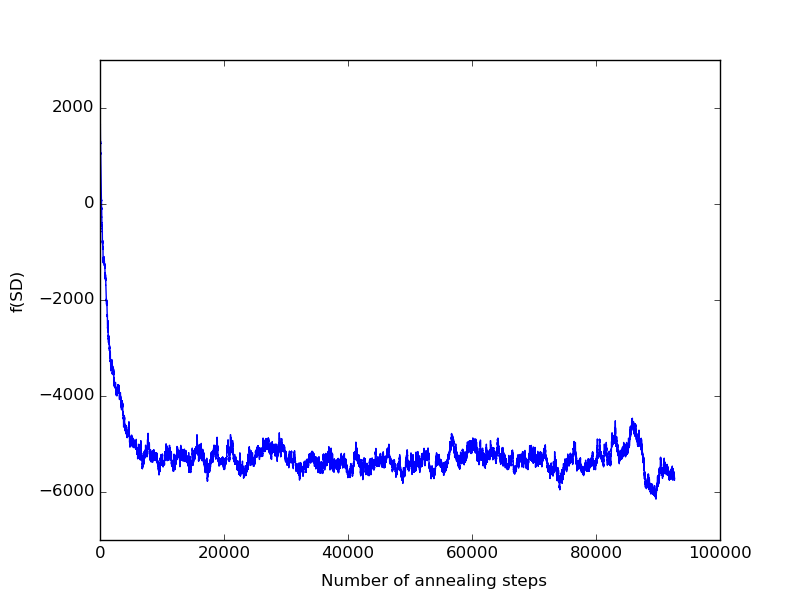
\includegraphics[scale=0.5]{figures/sa}
	\caption{Output of the simulated annealing algorithm graph-based
		\label{fig:saGraph}}
\end{figure}

Figure \ref{fig:saGraph} depicts the results of simulated annealing
using a graph-based neighborhood selection. It shows that the output
value progresses in an inverted exponential manner until it converges
to a certain value. At approximately 90000 steps a global optimum was
found. It is not known, however, whether this is the only optimum
(i.e. lowest energy state) or if there would be another optimum at a
later time.


\begin{algorithm}[htb]
	\caption{Simulated Annealing}\label{alg:sa}
	\begin{algorithmic}
		\Function{doSimulatedAnnealing}{}
		\State $current \gets initial()$
		\State $best \gets current$
		\While{$temp \geq 1$}			
		\If {$msteps = 0$} 
		\State $T \gets decreaseT()$
		\State $msteps \gets mstepsInit$
		\EndIf
		\State $new \gets \textsc{neighbor}(current)$
		\State $accept = e^{\frac{f(current)-f(new)}{T}}$
		\If {$f(new) < f(current)$}
		\State $current \gets new$
		\If {$f(new) < f(best)$}
		\State $best \gets new$
		\EndIf
		\ElsIf {$accept > random(0,1)$}
		\State $current \gets new$
		\EndIf		
		\EndWhile
		\State \Return $best$
		\EndFunction
		\Function{neighbor}{state}
		\State $node \gets selectRandomNode(state)$
		\State $child \gets selectRandomChild(node)$
		\State $state \gets changeValue(node)$
		\If {$exists(child)$}
		\State $state \gets changeValue(child)$
		\EndIf
		\State $state \gets changeValue(node)$
		\State \Return $state$
		\EndFunction
	\end{algorithmic}
\end{algorithm}
\section{Quantum Annealing}
\section{Experiments}
%
The experiment was performed on a single Intel Xeon CPU with 3.3 GHz
and 1.5 TB RAM, running a 64-Bit Ubuntu 14.04. As test instances the
ISCAS85 benchmark is used.

\subsection{Benchmark}
We used the ISCAS85 benchmark \cite{iscas} as the input to the
algorithms. The ISCAS85 benchmark consists several combinatorial
circuits that can be used to measure the performance of testing and
diagnosis algorithms. Included in the benchmark are circuits such as
decoders, multipliers, cryptography circuits, and arithmetic logic
units with the number of gates per circuit varying between 160 and
3512.

\subsection{Results}

Although the propositional logic formula that is used with SAFARI was
converted into a polynomial, the results show that the algorithms
specifically designed to work with propositional logic achieve far
better results than traditional optimization techniques using
polynomials. For all algorithms a fixed runtime was defined. Upon
exceeding the time limit the by then achieved parameters were taken as
the solution.

We define the following metric to denote the quality of a solution:
\emph{Isolation accuracy} $M_{ia} $ describes the quality of a
solution given the health state $H = \{\pr{f = \perp}\}$ (Definition
\ref{def:he}) and a fault injection $\phi$. We calculate the Euclidean
distance between $H$ and $\phi$ to determine how close the output of
an algorithm is to the original fault injection \cite{stern2015many}.

\begin{equation}
M_{ia} = \sqrt{\sum_{i=1}^{|H|} (\pr{f_i = \perp} - \pr{p_i = \perp})^2}
\end{equation}

With $f_i \in H$ and $p_i \in \phi$ and $M_{ia} \in
\mathcal{R}$. Smaller values of $M_{ia}$ indicate that the calculated
health state is closer to the fault injection. From this we can see
how good the diagnosis algorithm was able to determine the actual
injected fault. Bigger values on the other hand indicate that the
algorithm found more root-causes for faults than were in the
fault-injection $\phi$, which means that false-positive diagnoses are
generated.

Table~\ref{tbl:resGraph} shows the results the two approaches to
simulated annealing. The initial temperature was chosen in order to
achieve a reasonable probability for accepting worse states during
cool-down of the annealing algorithm. The number of steps indicates
how many annealing steps the algorithm performs until the temperature
is decreased. The number of iterations specifies how often the
algorithm was started for a specific observation $\alpha$ and a given
polynomial $p$. The outcome of the SA algorithm is the average value
of all iterations. From the table it can be concluded that the more
iterations are performed, the better the isolation accuracy
becomes. This can be explained through statistical analysis. As the
average value for determining the accuracy becomes closer to the real
value, the more iterations are performed.

Contrary to the assumption neither implementation of simulated
annealing is able to beat SAFARI in terms of speed or accuracy. While
isolation accuracy for simulated annealing is around 32 and 20,
respectively, SAFARI achieves an isolation accuracy of approximately
3. For these instances Random Search achieves an accuracy of
approximately 10. The low value of isolation accuracy for Random
Search can be explained through the algorithms ``lucky'' guessing and
finding a good solution given a sufficient amount of runs. For
simulated annealing on the other hand we can guarantee that it will
hit a global optimum eventually.
\begin{table*}[htb]
	\centering	
	\begin{tabular}{|l|l|c|c|c|c|c|}
		\hline
		\multicolumn{2}{|l|}{}                                                       & \textbf{Run 1} & \textbf{Run 2} & \textbf{Run 3} & \textbf{Run 4} & \textbf{Run 5} \\ \hline
		\multicolumn{1}{|c|}{\multirow{4}{*}{Parameters}} & \textbf{Temperature}     & 20             & 20             & 30             & 10             & 10             \\ \cline{2-7} 
		\multicolumn{1}{|c|}{}                            & \textbf{Steps}           & 10             & 4              & 20             & 20             & 5              \\ \cline{2-7} 
		\multicolumn{1}{|c|}{}                            & \textbf{Runtime}         & 20             & 20             & 60             & 20             & 20             \\ \cline{2-7} 
		\multicolumn{1}{|c|}{}                            & \textbf{Iterations}      & 5              & 5              & 5              & 50             & 50             \\ \hline
		\multirow{2}{*}{SA Graph}                         & \textbf{Steps completed} & 900          & 1800          & 95000         & 47000          & 45000            \\ \cline{2-7} 
		& \textbf{Isolation acc.}  & 32.4          &    32.3       & 31.4           & 32.2           & 32.8         \\ \hline
		\multirow{2}{*}{SA Random}                        & \textbf{Steps completed} & 800          & 1700          & 85000          & 42000          & 42000\\ \cline{2-7} 
		& \textbf{Isolation acc.}  & 20.1         & 19.9          & 19.6          & 20.0           & 20.0           \\ \hline
	\end{tabular}
	\caption{Runs with different parameters for simulated annealing using either the graph-based neighborhood selection (SA Graph) or a random selection of nodes (SA Random).\label{tbl:resGraph}}
\end{table*}
\begin{figure}[htb]
\centering
\includegraphics[scale=0.5]{multiplier.mps}
\caption{$n$-bit parallel multiplier\label{fig:multiplier}}
\end{figure}
%
\section{Related Work}
\section{Conclusions}

\end{document}
